\begin{figure}[t]
\centering
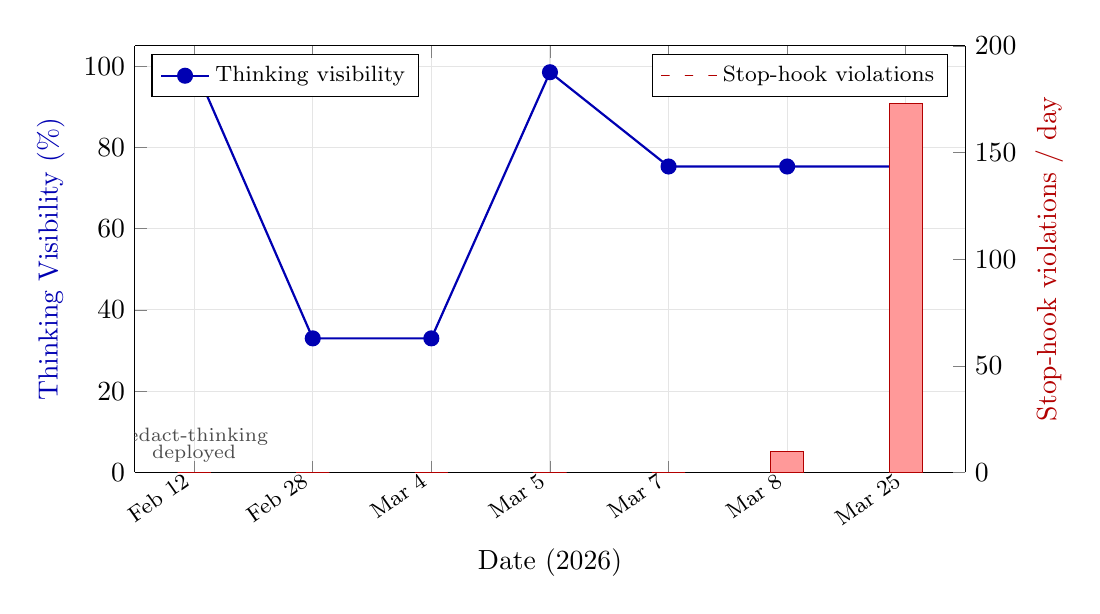
\begin{tikzpicture}
\begin{axis}[
    width=\textwidth,
    height=7cm,
    axis y line*=left,
    xlabel={Date (2026)},
    ylabel={Thinking Visibility (\%)},
    ylabel style={color=blue!70!black},
    ymin=0, ymax=105,
    xtick={1,2,3,4,5,6,7},
    xticklabels={Feb 12, Feb 28, Mar 4, Mar 5, Mar 7, Mar 8, Mar 25},
    xticklabel style={rotate=35, anchor=east, font=\footnotesize},
    xmin=0.5, xmax=7.5,
    legend style={at={(0.02,0.98)}, anchor=north west, font=\footnotesize},
    grid=major,
    grid style={gray!20},
]
% Thinking visibility line (declining)
\addplot[
    color=blue!70!black,
    mark=*,
    thick,
    mark size=2.5pt,
] coordinates {
    (1, 100)
    (2, 33)
    (3, 33)
    (4, 98.5)
    (5, 75.3)
    (6, 75.3)
    (7, 75.3)
};
\addlegendentry{Thinking visibility}
\end{axis}

\begin{axis}[
    width=\textwidth,
    height=7cm,
    axis y line*=right,
    axis x line=none,
    ylabel={Stop-hook violations / day},
    ylabel style={color=red!70!black},
    ymin=0, ymax=200,
    xmin=0.5, xmax=7.5,
    xtick=\empty,
    legend style={at={(0.98,0.98)}, anchor=north east, font=\footnotesize},
]
% Stop-hook violations bars (rising)
\addplot[
    ybar,
    bar width=12pt,
    fill=red!40,
    draw=red!70!black,
] coordinates {
    (1, 0)
    (2, 0)
    (3, 0)
    (4, 0)
    (5, 0)
    (6, 10)
    (7, 173)
};
\addlegendentry{Stop-hook violations}

% Annotation: redact-thinking deployed
\node[font=\scriptsize, anchor=south, text=black!70] at (axis cs:1,8) {redact-thinking};
\node[font=\scriptsize, anchor=south, text=black!70] at (axis cs:1,0) {deployed};

\end{axis}
\end{tikzpicture}
\caption{Timeline of behavioral degradation in the AMD dataset. Left axis: percentage of thinking content visible to the model (blue line). Right axis: stop-hook violations per day (red bars). The \texttt{redact-thinking} deployment on Feb~12 preceded a 67\% drop in thinking depth by late February. After partial visibility restoration on Mar~5, stop-hook violations surged from 0 to 173 over 17~days. Data from Laurenzo~\cite{laurenzo2026amd,laurenzo2026gist}.}
\label{fig:amd-timeline}
\end{figure}
